% Options for packages loaded elsewhere
\PassOptionsToPackage{unicode}{hyperref}
\PassOptionsToPackage{hyphens}{url}
%
\documentclass[
]{article}
\usepackage{amsmath,amssymb}
\usepackage{iftex}
\ifPDFTeX
  \usepackage[T1]{fontenc}
  \usepackage[utf8]{inputenc}
  \usepackage{textcomp} % provide euro and other symbols
\else % if luatex or xetex
  \usepackage{unicode-math} % this also loads fontspec
  \defaultfontfeatures{Scale=MatchLowercase}
  \defaultfontfeatures[\rmfamily]{Ligatures=TeX,Scale=1}
\fi
\usepackage{lmodern}
\ifPDFTeX\else
  % xetex/luatex font selection
\fi
% Use upquote if available, for straight quotes in verbatim environments
\IfFileExists{upquote.sty}{\usepackage{upquote}}{}
\IfFileExists{microtype.sty}{% use microtype if available
  \usepackage[]{microtype}
  \UseMicrotypeSet[protrusion]{basicmath} % disable protrusion for tt fonts
}{}
\makeatletter
\@ifundefined{KOMAClassName}{% if non-KOMA class
  \IfFileExists{parskip.sty}{%
    \usepackage{parskip}
  }{% else
    \setlength{\parindent}{0pt}
    \setlength{\parskip}{6pt plus 2pt minus 1pt}}
}{% if KOMA class
  \KOMAoptions{parskip=half}}
\makeatother
\usepackage{xcolor}
\usepackage[margin=1in]{geometry}
\usepackage{color}
\usepackage{fancyvrb}
\newcommand{\VerbBar}{|}
\newcommand{\VERB}{\Verb[commandchars=\\\{\}]}
\DefineVerbatimEnvironment{Highlighting}{Verbatim}{commandchars=\\\{\}}
% Add ',fontsize=\small' for more characters per line
\usepackage{framed}
\definecolor{shadecolor}{RGB}{248,248,248}
\newenvironment{Shaded}{\begin{snugshade}}{\end{snugshade}}
\newcommand{\AlertTok}[1]{\textcolor[rgb]{0.94,0.16,0.16}{#1}}
\newcommand{\AnnotationTok}[1]{\textcolor[rgb]{0.56,0.35,0.01}{\textbf{\textit{#1}}}}
\newcommand{\AttributeTok}[1]{\textcolor[rgb]{0.13,0.29,0.53}{#1}}
\newcommand{\BaseNTok}[1]{\textcolor[rgb]{0.00,0.00,0.81}{#1}}
\newcommand{\BuiltInTok}[1]{#1}
\newcommand{\CharTok}[1]{\textcolor[rgb]{0.31,0.60,0.02}{#1}}
\newcommand{\CommentTok}[1]{\textcolor[rgb]{0.56,0.35,0.01}{\textit{#1}}}
\newcommand{\CommentVarTok}[1]{\textcolor[rgb]{0.56,0.35,0.01}{\textbf{\textit{#1}}}}
\newcommand{\ConstantTok}[1]{\textcolor[rgb]{0.56,0.35,0.01}{#1}}
\newcommand{\ControlFlowTok}[1]{\textcolor[rgb]{0.13,0.29,0.53}{\textbf{#1}}}
\newcommand{\DataTypeTok}[1]{\textcolor[rgb]{0.13,0.29,0.53}{#1}}
\newcommand{\DecValTok}[1]{\textcolor[rgb]{0.00,0.00,0.81}{#1}}
\newcommand{\DocumentationTok}[1]{\textcolor[rgb]{0.56,0.35,0.01}{\textbf{\textit{#1}}}}
\newcommand{\ErrorTok}[1]{\textcolor[rgb]{0.64,0.00,0.00}{\textbf{#1}}}
\newcommand{\ExtensionTok}[1]{#1}
\newcommand{\FloatTok}[1]{\textcolor[rgb]{0.00,0.00,0.81}{#1}}
\newcommand{\FunctionTok}[1]{\textcolor[rgb]{0.13,0.29,0.53}{\textbf{#1}}}
\newcommand{\ImportTok}[1]{#1}
\newcommand{\InformationTok}[1]{\textcolor[rgb]{0.56,0.35,0.01}{\textbf{\textit{#1}}}}
\newcommand{\KeywordTok}[1]{\textcolor[rgb]{0.13,0.29,0.53}{\textbf{#1}}}
\newcommand{\NormalTok}[1]{#1}
\newcommand{\OperatorTok}[1]{\textcolor[rgb]{0.81,0.36,0.00}{\textbf{#1}}}
\newcommand{\OtherTok}[1]{\textcolor[rgb]{0.56,0.35,0.01}{#1}}
\newcommand{\PreprocessorTok}[1]{\textcolor[rgb]{0.56,0.35,0.01}{\textit{#1}}}
\newcommand{\RegionMarkerTok}[1]{#1}
\newcommand{\SpecialCharTok}[1]{\textcolor[rgb]{0.81,0.36,0.00}{\textbf{#1}}}
\newcommand{\SpecialStringTok}[1]{\textcolor[rgb]{0.31,0.60,0.02}{#1}}
\newcommand{\StringTok}[1]{\textcolor[rgb]{0.31,0.60,0.02}{#1}}
\newcommand{\VariableTok}[1]{\textcolor[rgb]{0.00,0.00,0.00}{#1}}
\newcommand{\VerbatimStringTok}[1]{\textcolor[rgb]{0.31,0.60,0.02}{#1}}
\newcommand{\WarningTok}[1]{\textcolor[rgb]{0.56,0.35,0.01}{\textbf{\textit{#1}}}}
\usepackage{longtable,booktabs,array}
\usepackage{calc} % for calculating minipage widths
% Correct order of tables after \paragraph or \subparagraph
\usepackage{etoolbox}
\makeatletter
\patchcmd\longtable{\par}{\if@noskipsec\mbox{}\fi\par}{}{}
\makeatother
% Allow footnotes in longtable head/foot
\IfFileExists{footnotehyper.sty}{\usepackage{footnotehyper}}{\usepackage{footnote}}
\makesavenoteenv{longtable}
\usepackage{graphicx}
\makeatletter
\newsavebox\pandoc@box
\newcommand*\pandocbounded[1]{% scales image to fit in text height/width
  \sbox\pandoc@box{#1}%
  \Gscale@div\@tempa{\textheight}{\dimexpr\ht\pandoc@box+\dp\pandoc@box\relax}%
  \Gscale@div\@tempb{\linewidth}{\wd\pandoc@box}%
  \ifdim\@tempb\p@<\@tempa\p@\let\@tempa\@tempb\fi% select the smaller of both
  \ifdim\@tempa\p@<\p@\scalebox{\@tempa}{\usebox\pandoc@box}%
  \else\usebox{\pandoc@box}%
  \fi%
}
% Set default figure placement to htbp
\def\fps@figure{htbp}
\makeatother
\setlength{\emergencystretch}{3em} % prevent overfull lines
\providecommand{\tightlist}{%
  \setlength{\itemsep}{0pt}\setlength{\parskip}{0pt}}
\setcounter{secnumdepth}{5}
\usepackage{booktabs}
\usepackage{longtable}
\usepackage{array}
\usepackage{multirow}
\usepackage{wrapfig}
\usepackage{float}
\usepackage{colortbl}
\usepackage{pdflscape}
\usepackage{tabu}
\usepackage{threeparttable}
\usepackage{threeparttablex}
\usepackage[normalem]{ulem}
\usepackage{makecell}
\usepackage{xcolor}
\usepackage[]{natbib}
\bibliographystyle{plainnat}
\nocite{*}
\usepackage{bookmark}
\IfFileExists{xurl.sty}{\usepackage{xurl}}{} % add URL line breaks if available
\urlstyle{same}
\hypersetup{
  pdftitle={SPUND-LX / AVL :: Appendix},
  pdfauthor={st. schwarz},
  hidelinks,
  pdfcreator={LaTeX via pandoc}}

\title{SPUND-LX / AVL :: Appendix}
\author{st. schwarz}
\date{2025-08-17}

\begin{document}
\maketitle

{
\setcounter{tocdepth}{2}
\tableofcontents
}
\section{index}\label{index}

linguistics, AVL, alii pub essais extension.

\begin{Shaded}
\begin{Highlighting}[]
\CommentTok{\#dataset\textless{}{-}7}
\end{Highlighting}
\end{Shaded}

\section{coherence \& proposition observations in :schizophrenia: threads}\label{coherence-proposition-observations-in-schizophrenia-threads}

eval output M12, normalised to obs, distance ceiling = outliers removed.

\subsection{citetest, method (M12)}\label{citetest-method-m12}

To compute distances we queried a corpus for matching conditions where certain (assumed) determiners appear before similar nouns. In M12 (removed)\ldots{} This distance should give us information structural evidence of how strong these noun occurences are connected, i.e.~if a noun appears out of the blue mostly or if it somewhere before has been introduced to the audience. In information structure definitions this would be termed with \textbf{given and new information} \citep{prince_toward_1981}.

\subsection{legende}\label{legende}

\begin{verbatim}
## [1] ", normalised to obs, distance ceiling =  outliers removed"
\end{verbatim}

\begin{longtable}[]{@{}
  >{\raggedright\arraybackslash}p{(\linewidth - 4\tabcolsep) * \real{0.1519}}
  >{\raggedright\arraybackslash}p{(\linewidth - 4\tabcolsep) * \real{0.5443}}
  >{\raggedright\arraybackslash}p{(\linewidth - 4\tabcolsep) * \real{0.3038}}@{}}
\caption{\label{tab:legend}model vars}\tabularnewline
\toprule\noalign{}
\begin{minipage}[b]{\linewidth}\raggedright
variable
\end{minipage} & \begin{minipage}[b]{\linewidth}\raggedright
explanation
\end{minipage} & \begin{minipage}[b]{\linewidth}\raggedright
values
\end{minipage} \\
\midrule\noalign{}
\endfirsthead
\toprule\noalign{}
\begin{minipage}[b]{\linewidth}\raggedright
variable
\end{minipage} & \begin{minipage}[b]{\linewidth}\raggedright
explanation
\end{minipage} & \begin{minipage}[b]{\linewidth}\raggedright
values
\end{minipage} \\
\midrule\noalign{}
\endhead
\bottomrule\noalign{}
\endlastfoot
target & corpus & obs,ref \\
q & condition & a,b,c,d,e,f \\
det & antecedent POS==DET & TRUE,FALSE \\
aut\_id & author & author hash \\
lemma & lemma & noun lemma \\
range & url range of distance devised & 1..maxlength(urlthread) \\
embed.score & semantic similarity score lemma vs.~thread & 0..1 \\
q:a & query condition & .* \\
q:b & query condition & this,that,those,these \\
q:c & query condition & the \\
q:d & query condition & a,an,any,some \\
q:e & query condition & my \\
q:f & query condition & his,her,their,your \\
\end{longtable}

\subsection{anova analysis}\label{anova-analysis}

\subsubsection{\texorpdfstring{anova plain, formula: {[}\texttt{dist\_rel\_obs\ \textasciitilde{}\ target*q*det}{]}}{anova plain, formula: {[}dist\_rel\_obs \textasciitilde{} target*q*det{]}}}\label{anova-plain-formula-dist_rel_obs-targetqdet}

\begin{verbatim}
##                   Df     Sum Sq    Mean Sq    F value Pr(>F)    
## target             1 6.5314e+09 6531359317 3.2559e+05 <2e-16 ***
## q                  5 3.5058e+08   70116374 3.4953e+03 <2e-16 ***
## det                1 1.5458e+07   15457530 7.7056e+02 <2e-16 ***
## target:q           5 1.8239e+06     364778 1.8184e+01 <2e-16 ***
## target:det         1 6.1232e+06    6123176 3.0524e+02 <2e-16 ***
## q:det              1 3.1197e+04      31197 1.5552e+00 0.2124    
## target:q:det       1 1.8157e+06    1815712 9.0514e+01 <2e-16 ***
## Residuals    2249061 4.5116e+10      20060                      
## ---
## Signif. codes:  0 '***' 0.001 '**' 0.01 '*' 0.05 '.' 0.1 ' ' 1
\end{verbatim}

\subsubsection{\texorpdfstring{anova of linear regression model: {[}\texttt{anova(summary(lmer))}{]}}{anova of linear regression model: {[}anova(summary(lmer)){]}}}\label{anova-of-linear-regression-model-anovasummarylmer}

\begin{verbatim}
## Type III Analysis of Variance Table with Satterthwaite's method
##                 Sum Sq   Mean Sq NumDF  DenDF    F value    Pr(>F)    
## target           82484     82484     1 155603     4.2727   0.03873 *  
## q              1614197    322839     5 155801    16.7235 < 2.2e-16 ***
## det              54104     54104     1 155344     2.8026   0.09411 .  
## range        250671788 250671788     1 151248 12985.0989 < 2.2e-16 ***
## embed.score    3797399   3797399     1 157460   196.7098 < 2.2e-16 ***
## target:q       1064174    212835     5 155772    11.0251 1.235e-10 ***
## target:det       30708     30708     1 156612     1.5907   0.20722    
## q:det           105369    105369     1 155289     5.4582   0.01948 *  
## target:q:det                                                          
## ---
## Signif. codes:  0 '***' 0.001 '**' 0.01 '*' 0.05 '.' 0.1 ' ' 1
\end{verbatim}

\subsubsection{\texorpdfstring{linear regression coefficients, formula: {[}\texttt{dist\_rel\_obs\ \textasciitilde{}\ target*q*det+(1\textbar{}aut\_id)+range+embed.score}{]}}{linear regression coefficients, formula: {[}dist\_rel\_obs \textasciitilde{} target*q*det+(1\textbar aut\_id)+range+embed.score{]}}}\label{linear-regression-coefficients-formula-dist_rel_obs-targetqdet1aut_idrangeembed.score}

\begin{verbatim}
## Linear mixed model fit by REML. t-tests use Satterthwaite's method [
## lmerModLmerTest]
## Formula: eval(expr(lmeform))
##    Data: dfa
## 
## REML criterion at convergence: 2014129
## 
## Scaled residuals: 
##     Min      1Q  Median      3Q     Max 
## -6.5794 -0.3429 -0.0365  0.1456 15.9844 
## 
## Random effects:
##  Groups   Name        Variance Std.Dev.
##  aut_id   (Intercept) 41939    204.8   
##  Residual             19305    138.9   
## Number of obs: 157757, groups:  aut_id, 2512
## 
## Fixed effects:
##                     Estimate Std. Error         df  t value Pr(>|t|)    
## (Intercept)        3.386e+02  4.772e+00  3.367e+03   70.953  < 2e-16 ***
## targetref         -1.375e+01  4.211e+00  3.588e+04   -3.266 0.001093 ** 
## qb                 6.711e+01  1.328e+01  1.553e+05    5.055 4.31e-07 ***
## qc                 4.929e+01  2.865e+00  1.553e+05   17.204  < 2e-16 ***
## qd                 5.424e+01  2.903e+00  1.554e+05   18.686  < 2e-16 ***
## qe                 8.939e+01  4.512e+00  1.555e+05   19.811  < 2e-16 ***
## qf                 7.966e+01  5.550e+00  1.554e+05   14.352  < 2e-16 ***
## detTRUE            5.402e+00  1.346e+00  1.562e+05    4.012 6.01e-05 ***
## range             -3.799e-02  3.334e-04  1.512e+05 -113.952  < 2e-16 ***
## embed.score        6.208e+01  4.426e+00  1.575e+05   14.025  < 2e-16 ***
## targetref:qb      -7.595e+01  3.371e+01  1.563e+05   -2.253 0.024268 *  
## targetref:qc      -4.976e+01  1.388e+01  1.551e+05   -3.585 0.000337 ***
## targetref:qd      -4.986e+01  1.283e+01  1.550e+05   -3.886 0.000102 ***
## targetref:qe      -1.036e+02  3.677e+01  1.575e+05   -2.816 0.004856 ** 
## targetref:qf       2.261e+02  5.835e+01  1.550e+05    3.876 0.000106 ***
## targetref:detTRUE -3.762e+00  2.982e+00  1.566e+05   -1.261 0.207223    
## qb:detTRUE        -3.566e+01  1.527e+01  1.553e+05   -2.336 0.019478 *  
## ---
## Signif. codes:  0 '***' 0.001 '**' 0.01 '*' 0.05 '.' 0.1 ' ' 1
## fit warnings:
## fixed-effect model matrix is rank deficient so dropping 9 columns / coefficients
## Some predictor variables are on very different scales: consider rescaling
\end{verbatim}

\subsection{plots}\label{plots}

\begin{figure}
\centering
\pandocbounded{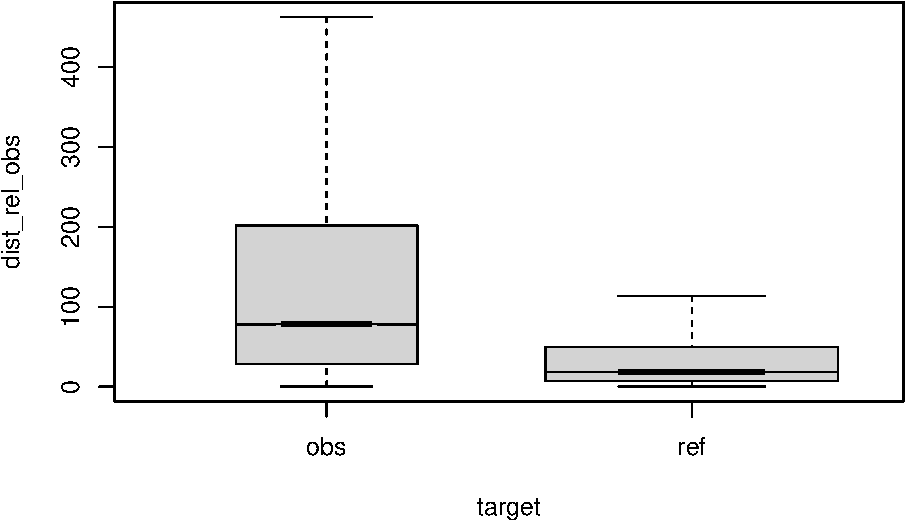
\includegraphics[keepaspectratio]{poster-ext_files/figure-latex/boxplot1-1.pdf}}
\caption{\label{fig:boxplot1}compare distances by corpus, normalised to obs, distance ceiling = outliers removed}
\end{figure}

\begin{figure}
\centering
\pandocbounded{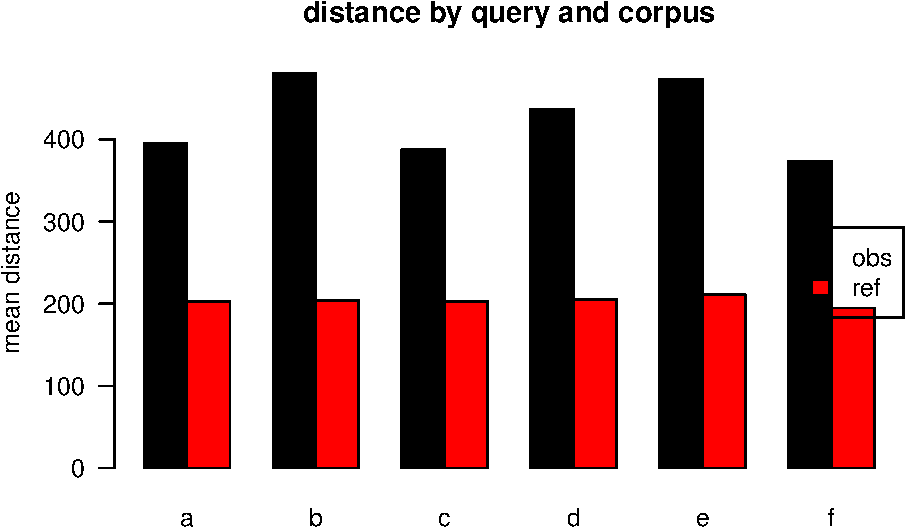
\includegraphics[keepaspectratio]{poster-ext_files/figure-latex/barplot-median-1.pdf}}
\caption{\label{fig:barplot-median}mean distances over query/corpus, normalised to obs, distance ceiling = outliers removed}
\end{figure}

\begin{longtable}[]{@{}llrrr@{}}
\caption{\label{tab:dfe-table}mean/median table for M12}\tabularnewline
\toprule\noalign{}
target & q & n & mean & median \\
\midrule\noalign{}
\endfirsthead
\toprule\noalign{}
target & q & n & mean & median \\
\midrule\noalign{}
\endhead
\bottomrule\noalign{}
\endlastfoot
obs & a & 541133 & 158 & 73 \\
ref & a & 1609781 & 45 & 18 \\
obs & b & 5540 & 196 & 108 \\
ref & b & 2407 & 94 & 70 \\
obs & c & 25564 & 219 & 125 \\
ref & c & 4550 & 90 & 54 \\
obs & d & 23803 & 228 & 132 \\
ref & d & 4498 & 114 & 63 \\
obs & e & 18067 & 238 & 131 \\
ref & e & 1417 & 123 & 80 \\
obs & f & 11464 & 189 & 104 \\
ref & f & 853 & 67 & 55 \\
\end{longtable}

\begin{figure}
\centering
\pandocbounded{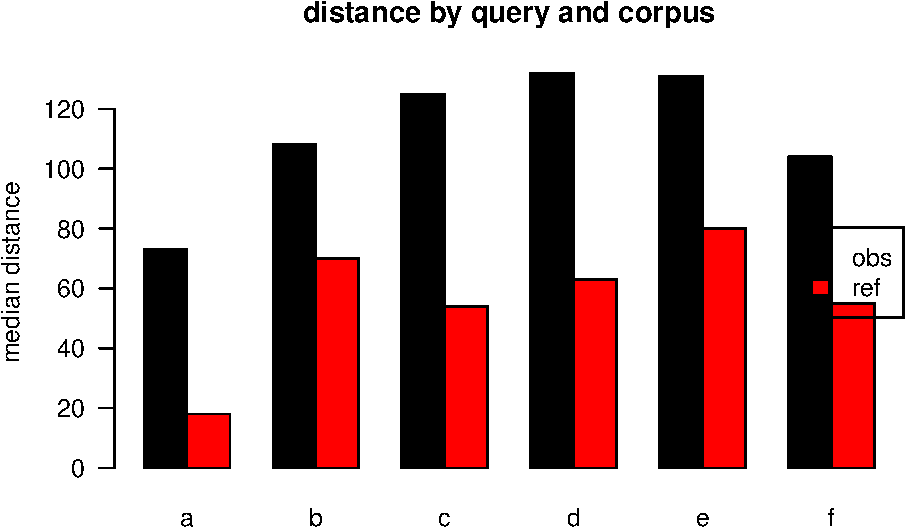
\includegraphics[keepaspectratio]{poster-ext_files/figure-latex/barplot-mean-1.pdf}}
\caption{\label{fig:barplot-mean}median distances over query/corpus, normalised to obs, distance ceiling = outliers removed}
\end{figure}

\begin{figure}
\centering
\pandocbounded{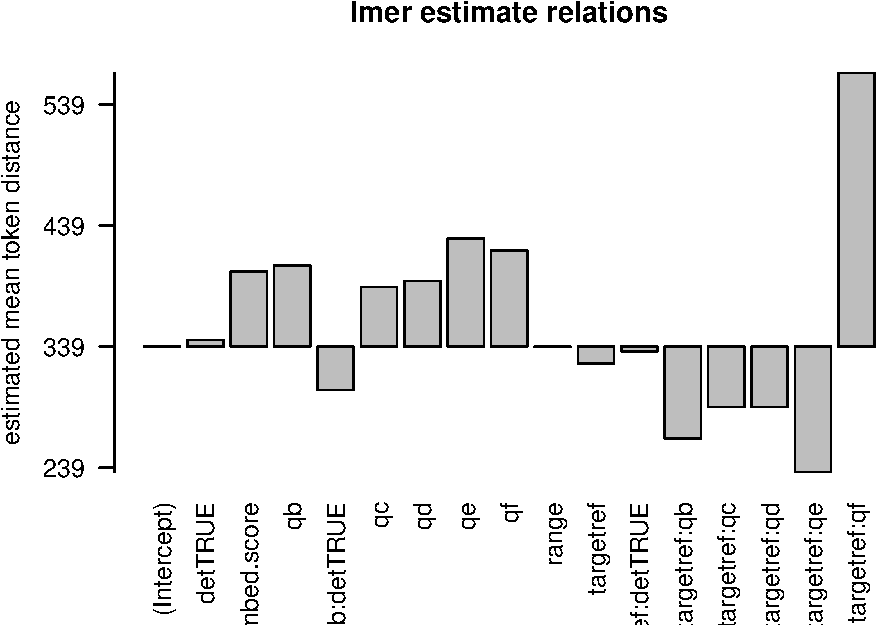
\includegraphics[keepaspectratio]{poster-ext_files/figure-latex/lmeplot-1.pdf}}
\caption{\label{fig:lmeplot}distances relation, normalised to obs, distance ceiling = outliers removed}
\end{figure}

\subsection{\texorpdfstring{\protect\pandocbounded{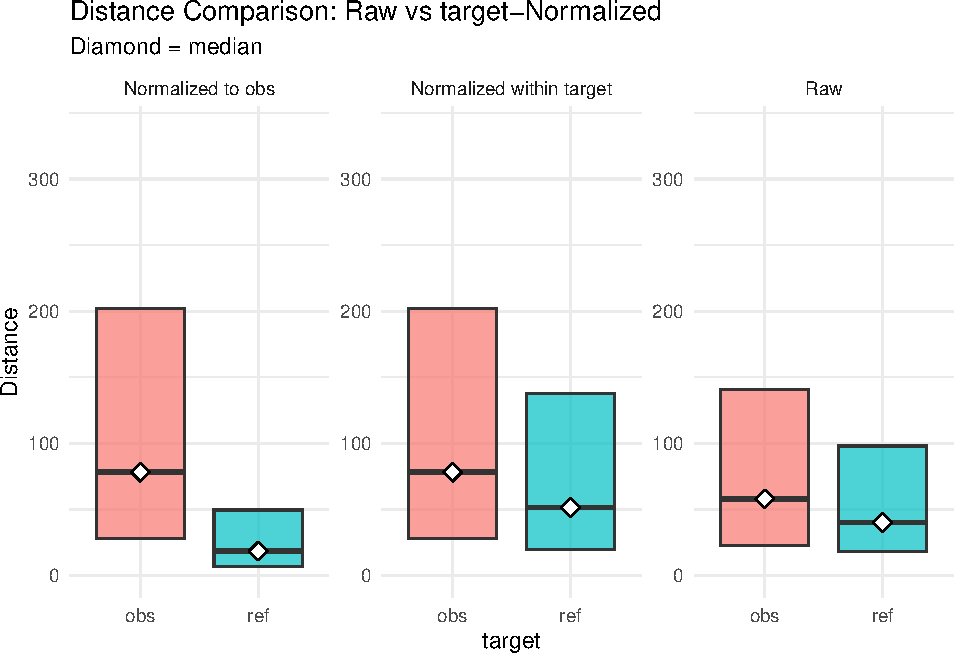
\includegraphics[keepaspectratio]{poster-ext_files/figure-latex/gplot-1.pdf}}}{\label{fig:gplot}distances normalised vs.~raw}}\label{figgplotdistances-normalised-vs.-raw}

\subsection{REF}\label{ref}

literature used and alii\ldots{}

\section{15303.paper.draft}\label{paper.draft}

\subsection{subject}\label{subject}

Investigate reference marking, coherence and information structure in schizophrenia language by measuring distance of similar nouns within range of comment thread preceded by certain determinants.\footnote{snc.1:h2.pb.1000char/pg.queries.cites}

\subsection{background}\label{background}

Inspired by Zimmerer et al.~(2017) we are interested in observations concerning coherence and propositional statement conditions in schizophrenia language, as these linguistic markers appear underinvestigated in that fields research whilst they seem to play a crucial role target group language features. (As such seen as asset of thinking or world building capacity which might suffer from linguistic deficits within the range of positive symptoms.)

\subsection{definitions}\label{definitions}

\subsubsection{coherence}\label{coherence}

There are several preliminary affordances to a successful communication. One is the \textbf{coherence} of a \hyperref[]{text = way of communication}, which accounts for the partner being able to follow the topic and relate subjects and objects referenced. There can be more or less \textbf{common} references and such, that need to be embedded in context to be understood. The underlying network of informations to create that context is what we call \textbf{information structure} of a text. The level of complexity of that network defines how simple it would be to gather the reference from the given information. We could have to go back many sentences or even infer reference from metaphors or such to be able to understand what is said or in the other case simply recall the subject of the last sentence to get the meaning (reference) of the pronoun in \texttt{also\ \{she\}\ said\ thisandthat...}.
The capacity to imagine or have in mind, what concrete information is accessible to the adressee (what he actually knows or can infer) is key to a successful communication, since factors like common knowledge, weltwissen and shared knowledge between adressant and adressee and information accessible from the text itself varies depending on topic, setting, intimacy of the partners and such. So one cannot always be sure that all information provided is sufficient, but the grade to which one can give the right estimate to this sufficiency should here be a measure for our hypothesis, that the very coherence in disturbed language is deficient such that an utterance is more difficult to understand within the frame of given information.
Now one indicator of that coherence we assume is \textbf{reference distance} where according to our hypothesis a larger distance would be observed in places where the adressant overestimates\footnote{due to lack of empathy or a general self-alignment} the ability of the partner to follow a reference. That would mean that we find a medium shorter distance between referent and reference in the reference corpus\footnote{where the participants may show a more realistic estimation of beforementioned ability} and larger distances in the target corpus. The references we are interested in are nouns that appear as anaphors i.e.~here as noun analogies. The assumption is that if a noun is repeated \textbf{and} is combinded with certain preceding determiners, the speaker assumes that the adressee has some knowledge of what is talked about, depending on the strength of the determination. So {[}this, that, those, these{]} would be rather strong determiners requiring that the noun most definitely was introduced before; these four determiners depict on of our 5 conditions listed below.

\subsection{questions}\label{questions}

Measuring the referent-reference distance which we assume as indicator of coherence we hope to find empirical evidence for disturbed or not world building capacities within schizophrenia language. Premising that a large noun distance indicates a low reference-referent association we hypothesise that in a language/ToM setting where the speakers estimation of the audiences context understanding capacities is disturbed we will find higer medium scores for the distance under matching conditions. An environment which has potential to test our hypothesis is the reddit thread r/schizophrenia. As reference corpus we chose reddit r/unpopularopinion.
The distance measured should give us information structural evidence of how strong the noun occurences\footnote{preceded by conditioned determiners} are connected, i.e.~if a noun appears out of the blue mostly or if it somewhere before has been introduced to the audience thus it will be more or less legitimated to be determined by an antecedent. In information structure definitions we here rely on the terms \textbf{given and new information} coined by (Prince 1981).

\subsection{daten}\label{daten}

We built a corpus of the reddit r/schizophrenia thread (\texttt{n=755074} tokens) and a reference corpus of r/unpopularopinion (\texttt{n=271563}). Both were pos-tagged using the R udpipe package (Wijffels 2023) which tags according to the universal dependencies tagset maintained by De Marneffe et al.~(2021). Still the 755074 tokens can only, within the workflow of growing the corpus and devising the noun distances developed be just a starting point from where with more datapoints statistical evaluation becomes relevant first.\\
The dataframe used for our model (actual: MX) consists of \texttt{939879} distance datapoints (sample Tab.X) derived from the postagged corpus.

\subsection{methods}\label{methods}

To compute distances we queried the corpus for matching conditions where certain (probable) determiners appear before analogue nouns (anaphors). For each datapoint we collect variables as:
- thread url
- author (anonymised)
- thread length (tokens)
- lexical diversity (type/token ratio)
- lemma
- distance (to the preceding occurence, e.g.~for three occurences of {[}dog{]} we collect 2 distance datapoints)

The main function to determine the distances runs on a subset of the corpus with only including all nouns and their position in the corpus. It finds all duplicated nouns per url thread and computes their distances by token position.

\subsection{reflections}\label{reflections}

\subsubsection{range}\label{range}

Evaluating with a growing corpus and (reaching up to M{[}odel{]}12 with our methods of computing distances) we interestingly find our basic hypothesis tested again, showing an overall larger distance of analogue nouns within the range of 1 thread url for the target corpus. While until M7 we devised distances from a manually assigned url identifier we saw the necessity to define our ``range of interest'' according to the original http url of the thread, since with a growing corpus the old url ids, derived from the get\_thread\_url() method of the redditExtractoR: package, there a no new url ids created since one url fetch gets each time always only around 1000 urls. To ensure unique url ranges within the corpus we as said in M11 assigned the range (within which the noun distance is calculated) to the real thread url. The corpus itself is after each fetch sorted after url and timestamp so it represents the real flow of conversation within one thread which is important since our distance model is based on the token distances within that thread, so they should follow their natural occurence in time.

\subsubsection{author trace id}\label{author-trace-id}

Another nice new feature in M11 is the aut\_id variable which represents the comment author and is unique to that. In the base .sqlite database the authors are already anonymised, so there should be no way from the published data back to the original author name of the comment. But, as also expected, including aut\_id as random effect in the linear regression model, the significance level for the covariables of interest as are
1. q = the condition matching of the noun-preceding token
2. det = wether that match has postag ``DET''
3. target = obs or reference corpus
finally increases.

\subsubsection{lexical diversity}\label{lexical-diversity}

We thought about some serious caveats within the latest method: If (lucky for our hypothesis) the target corpus has significantly higher distance scores over nearly all conditions, does that automatically indicate a less coherent reference-referent association within what is expressed in the comments? Couldn't we also assume that if the analogue nouns appear more distanced in general that a topic which is including these nouns is simply expanding over a wider range i.e.~timeframe? What does that do to our assumptions in terms of coherence? A good way here could be to integrate (from M3) a general lexical diversity factor per url as fixed effect because we can assume that a higher type/token ratio logically decreases the probability of a noun appearing multiple times within a range and we could take that effect into account.

\subsubsection{semantics, word field, embedding}\label{semantics-word-field-embedding}

Further we created another covariable possible to integrate in the evaluation model: The probability of one specific noun appearing on its specific position in the thread range, computed with help of an open LL word embedding model{[}\#ref{]}. This is a common AI way of devising semantic relations in a corpus which exceeds a just frequency based keyword analysis. Using an LLM here allows for a distinctive identification of world field embeddings of the noun in question. In that way we get another variable linguistic feature extracted which may give general insights into the level of standardisation that applies to the corpora. So if a noun is found to be embedded with a high score into its context (the url thread) then it can be very much expected to be found there and does not appear out-of-context.\footnote{only according to the LLM training data, which is still a blackbox}

\subsection{caveats}\label{caveats}

Since devising the word embed score does take much computing ressources we had a script run on a server that solves the computing. But the first essai to integrate the new var into the evaluation model failed due to levels \textless{} 2. Why? Because since we ran the script over the complete url ranges in the corpus and that is sorted after target,\footnote{where ``obs'' comes first} we did not compute any values for the reference corpus. So we learned this way again on linear regression models which require that a variable has more than one level (which would not be the case if the lmer() function excludes all NA rows: there will be no observations left with target=ref since all its embed.score values are NA and so all target.ref rows will be removed during regression.

\begin{center}\rule{0.5\linewidth}{0.5pt}\end{center}

\subsection{REF}\label{ref-1}

literature used and alii\ldots{}

\section{R Markdown template page, first h1}\label{r-markdown-template-page-first-h1}

\begin{itemize}
\tightlist
\item
  test for yaml title
\end{itemize}

This is an R Markdown document. Markdown is a simple formatting syntax for authoring HTML, PDF, and MS Word documents. For more details on using R Markdown see \url{http://rmarkdown.rstudio.com}.

When you click the \textbf{Knit} button a document will be generated that includes both content as well as the output of any embedded R code chunks within the document. You can embed an R code chunk like this:

\begin{Shaded}
\begin{Highlighting}[]
\FunctionTok{summary}\NormalTok{(cars)}
\end{Highlighting}
\end{Shaded}

\begin{verbatim}
##      speed           dist       
##  Min.   : 4.0   Min.   :  2.00  
##  1st Qu.:12.0   1st Qu.: 26.00  
##  Median :15.0   Median : 36.00  
##  Mean   :15.4   Mean   : 42.98  
##  3rd Qu.:19.0   3rd Qu.: 56.00  
##  Max.   :25.0   Max.   :120.00
\end{verbatim}

\begin{Shaded}
\begin{Highlighting}[]
\NormalTok{knitr}\SpecialCharTok{::}\FunctionTok{kable}\NormalTok{(}\FunctionTok{head}\NormalTok{(cars))}
\end{Highlighting}
\end{Shaded}

\begin{tabular}{r|r}
\hline
speed & dist\\
\hline
4 & 2\\
\hline
4 & 10\\
\hline
7 & 4\\
\hline
7 & 22\\
\hline
8 & 16\\
\hline
9 & 10\\
\hline
\end{tabular}

\section{Including Plots}\label{including-plots}

You can also embed plots, for example:

\pandocbounded{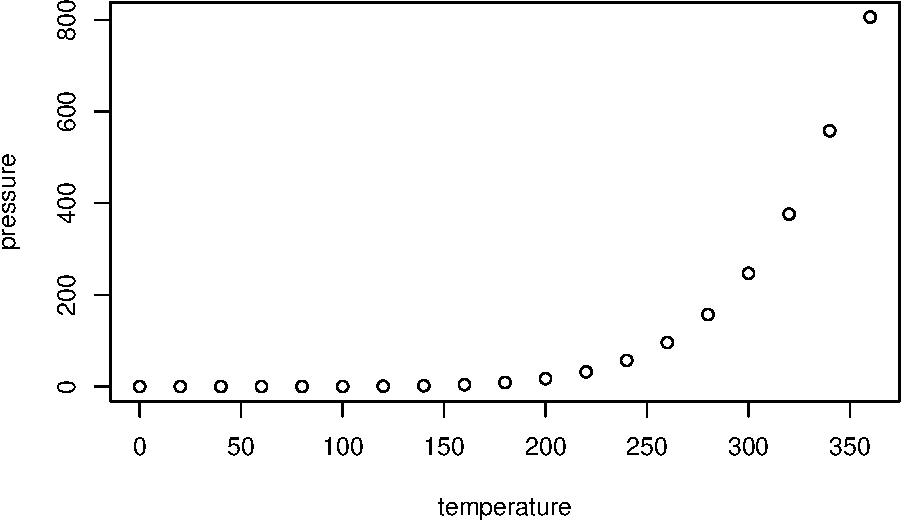
\includegraphics[keepaspectratio]{testpages_files/figure-latex/pressure-1.pdf}}

Note that the \texttt{echo\ =\ FALSE} parameter was added to the code chunk to prevent printing of the R code that generated the plot.

\subsection{quellen da?}\label{quellen-da}

\begin{center}\rule{0.5\linewidth}{0.5pt}\end{center}

\section{REF global}\label{ref-global}

  \bibliography{psych.bib}

\end{document}
